% -*- TeX-master: "main"; fill-column: 72 -*-

\section{Illustrative examples of the \Render syntax}
\label{examples}


This is an example on how an SBGN document could be represented using the SBML layout and render extensions. The example represented once as an SBML Level 2 Version 1 document using annotations and once as an SBML Level 3 Version 1 document with the layout and render extension packages.

The example contains only one simple layout and three global as well as one local style.
Although this example does not show all features of the render extension, it should give a good overview on how the layout and the render extension are used together.

The following four figures are generated from this example using the xslt style sheet implementation with xsltproc.
The SVG images were then rendered with the Chrome Browser from Google.

\begin{figure}[!h]
\begin{center}
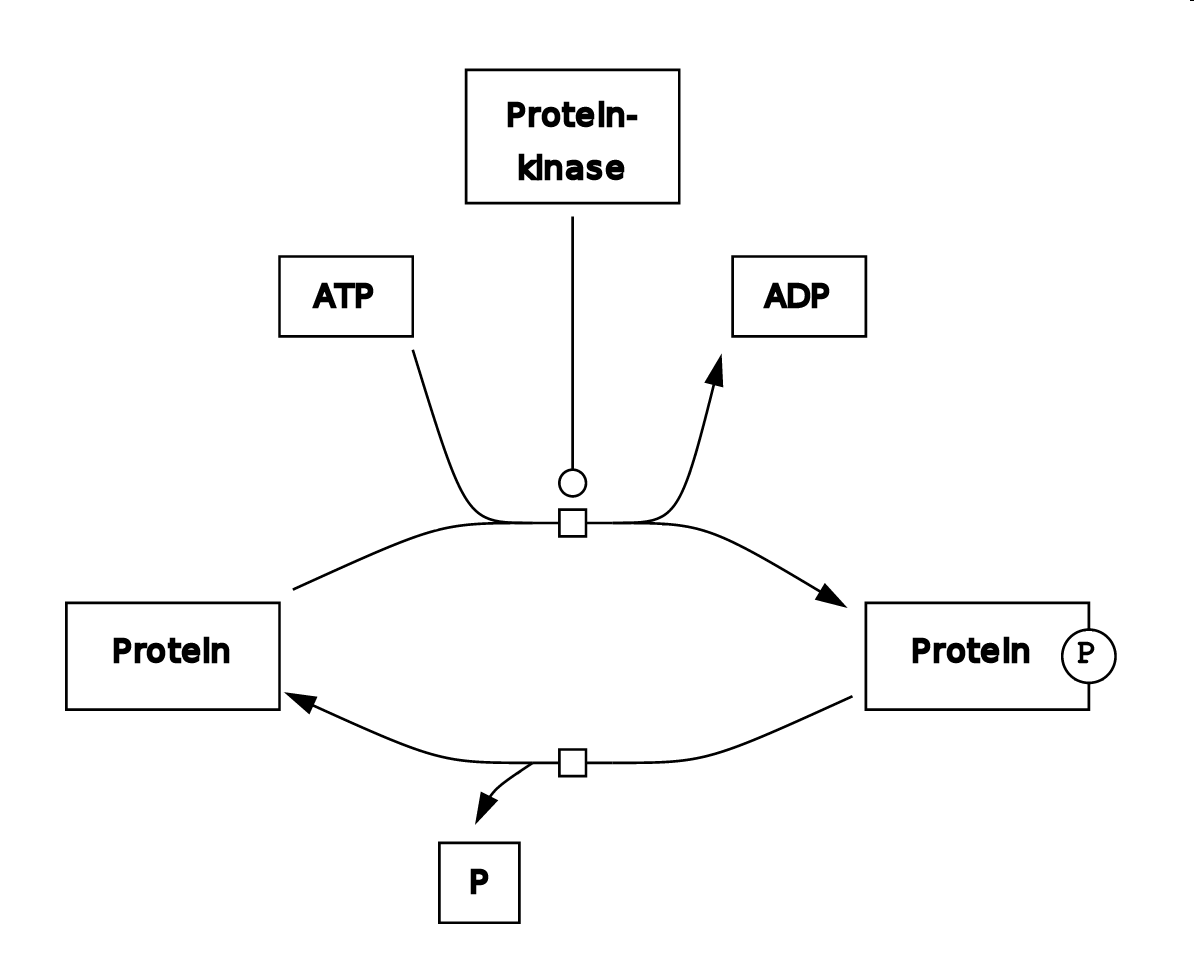
\includegraphics[width=0.4\textwidth]{figures/Phosphorylation_wireFrame}
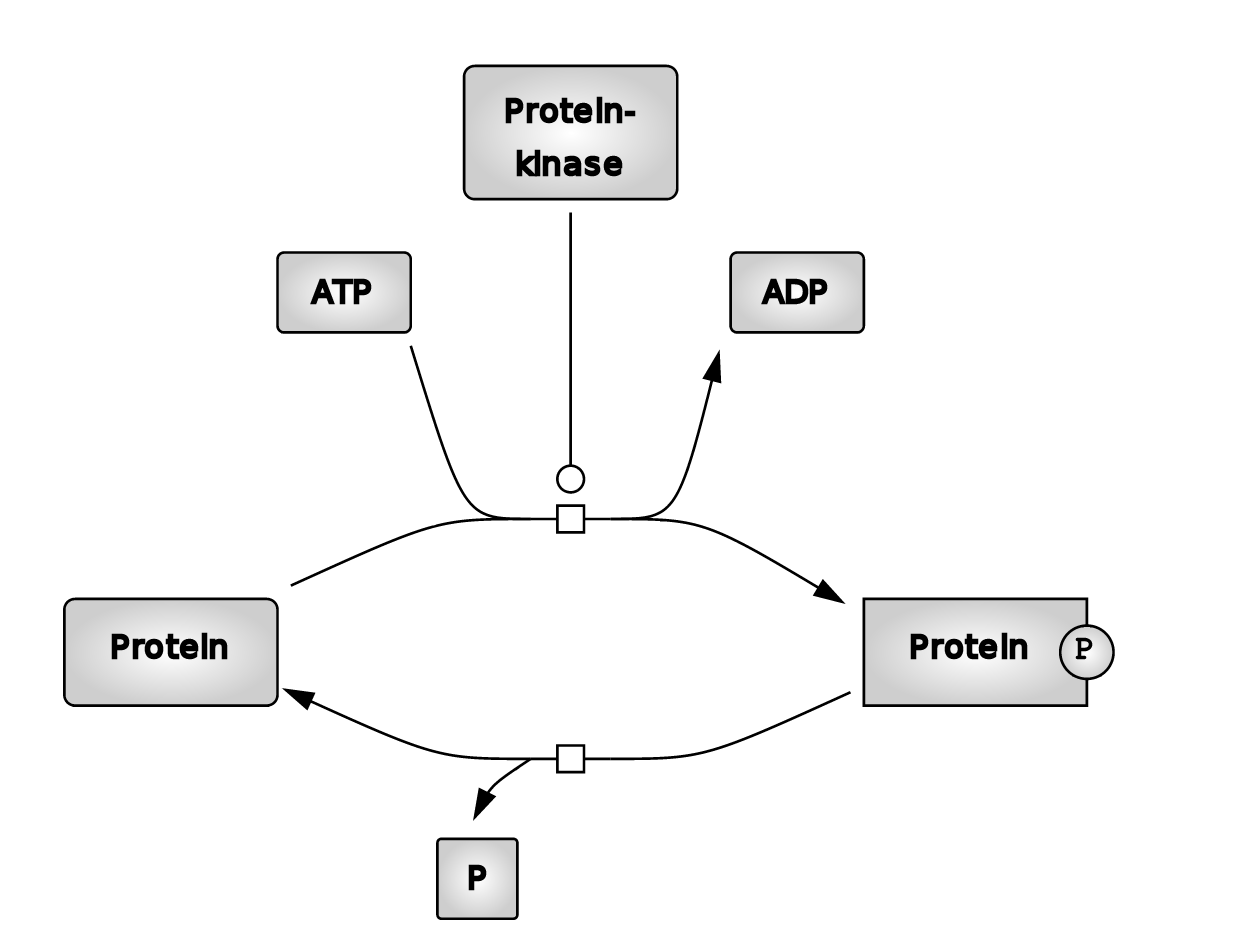
\includegraphics[width=0.4\textwidth]{figures/Phosphorylation_gray}
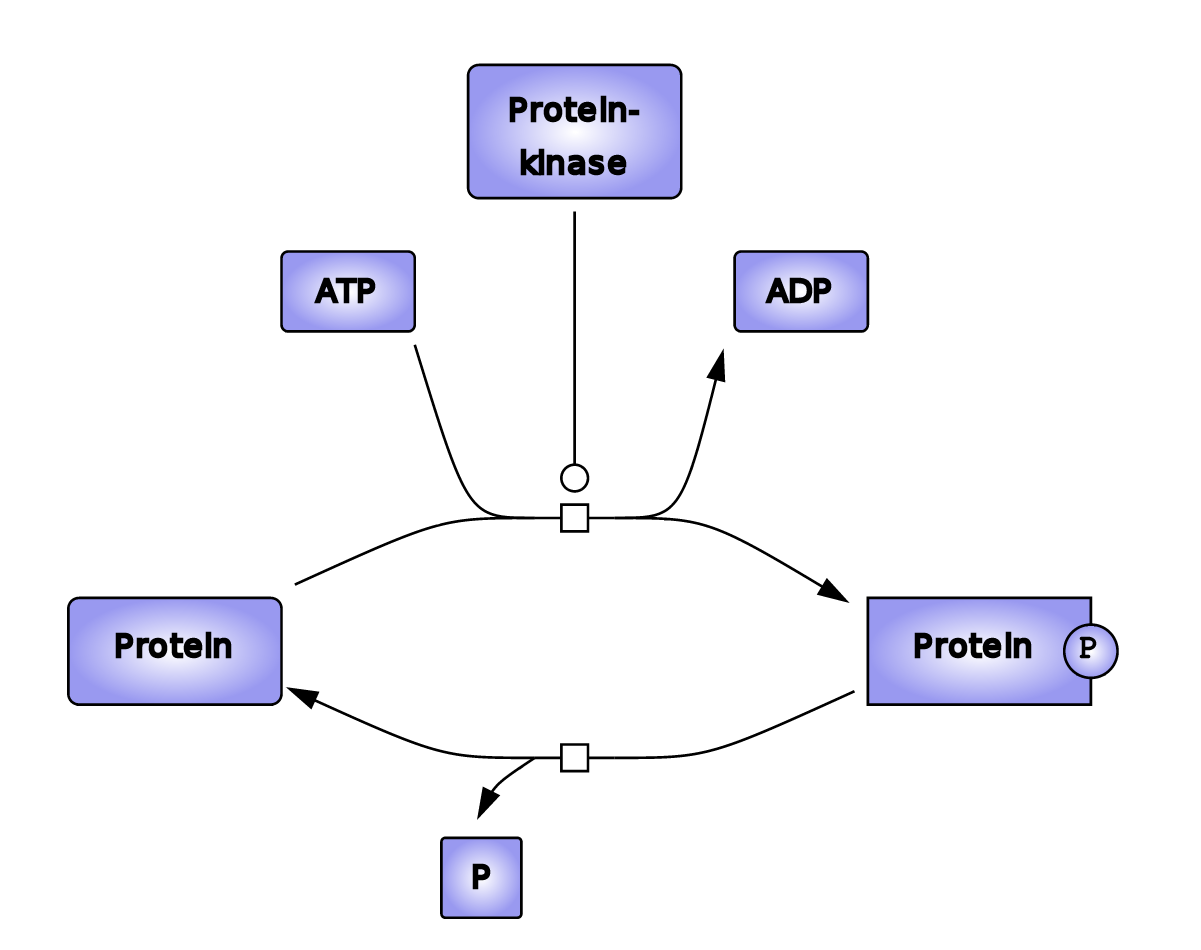
\includegraphics[width=0.4\textwidth]{figures/Phosphorylation_color}
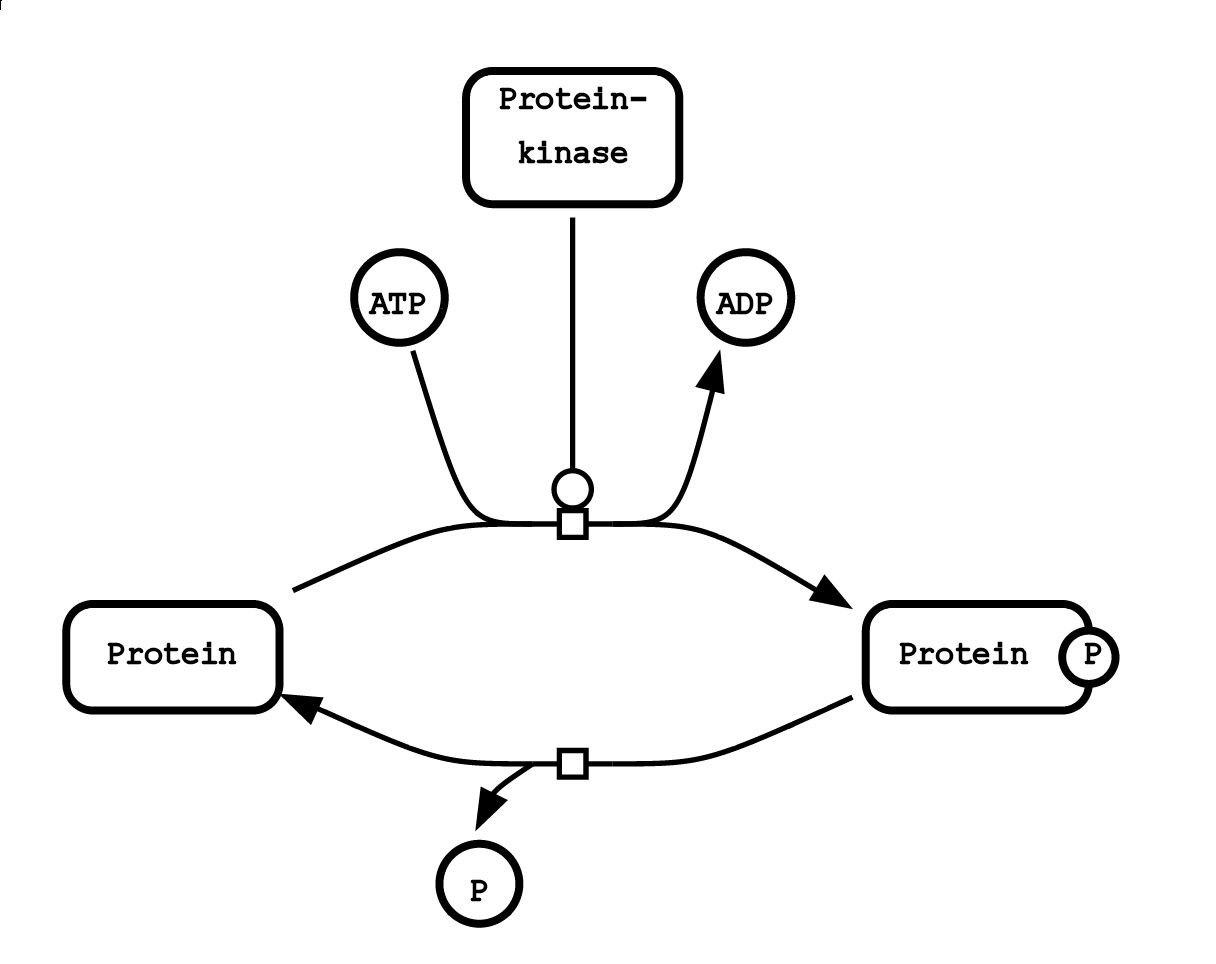
\includegraphics[width=0.4\textwidth]{figures/Phosphorylation_SBGN}
\end{center}
\caption{example converted to SVG and rendered with Google Chrome browser}
\label{ExampleRendering}
\end{figure}



\subsection*{SBML Level 3 Version 1}

\exampleFile{examples/example_l3v1_fixed.xml}

\subsection*{SBML Level 2 Version 1}

%\lstset{language=XML,tabsize=1,basicstyle=\footnotesize,breaklines=true}

\exampleFile{examples/example_l2v1_fixed.xml}



